\documentclass[11pt]{article}
\usepackage[utf8]{inputenc}
\usepackage[english]{babel}
\usepackage{bilal2vec}

\title{SE 380 — HW 2}
\author{Bilal Khan\\
\href{mailto:bilal2vec@gmail.com}{bilal2vec@gmail.com}}
\date{\today}

\begin{document}

\maketitle

\tableofcontents

\section{1}

\subsection{a}

Considering the state space model

\begin{align*}
    \dot{x} &= Ax + Bu \\
    y &= Cx + Du
\end{align*}

where $x \in \mathbb{R}^2$, $u \in \mathbb{R}^2$, and $y \in \mathbb{R}$, find values for $A, B, C, D$ such that the corresponding transfer function is

\begin{align*}
    G(s) &= \dfrac{\mu}{1 + \tau s} \\
\end{align*}

Taking the Laplace transform of the above equations, we get

\begin{align*}
    sX(s) - x(0) &= AX(s) + BU(s) \\
    Y(s) &= CX(s) + DU(s)
\end{align*}

Solving this, assuming initial state is zero, we get

\begin{align*}
    sX(s) - x(0) &= AX(s) + BU(s) \\
    sX(s) - AX(s) &= BU(s) \\
    X(s) (sI - A) &= BU(s) \\
    X(s) &= \dfrac{BU(s)}{sI - A} \\
    Y(s) &= \left( \dfrac{CB}{sI - A} + D \right) U(s) \\
    H(S) &= \dfrac{Y(s)}{U(s)} = \dfrac{CB}{sI - A} + D \\
    \dfrac{CB}{sI - A} &= \dfrac{\mu}{1 + \tau s}
\end{align*}

We want $CB = \mu$, so one possible solution is

\[
    C = \begin{bmatrix} \mu & 0 \end{bmatrix} \\
    B = \begin{bmatrix} 1 \\ 0 \end{bmatrix}
\]

The $1 + \tau s$ term can be made simpler by rearranging it to $s + \frac{1}{\tau}$, and we want the same $x_1(t)$ state value to change as in $B$ so we want $A$ to be

\[
    A = \begin{bmatrix}
        -\dfrac{1}{\tau} & 0 \\
        0 & 0 \\ 
    \end{bmatrix}
\]

$D$ is zero because we do not use it in the transfer function.

\subsection{b}

No, there are multiple ways to set up the state space matrices to get the same transfer function. For example, we could have chosen $x_2(t)$ to be the state variable we use and then choose $C$ to be $\begin{bmatrix} 0 & \mu \end{bmatrix}$ and $B$ to be $\begin{bmatrix} 0 \\ 1 \end{bmatrix}$, and $A$ to be $\begin{bmatrix} 0 & 0 \\ -\dfrac{1}{\tau} & 0 \end{bmatrix}$, and $D$ to be zero. This would have given us the same transfer function.

\section{2}

\subsection{a}

Consider a first-order system with transfer function given by $H(s) = \dfrac{\mu}{1 + \tau s}$. Compute the response $y_1(t)$ to a step input $u_1(t) = H(t)$ and the response of $y_2(t)$ to a ramp input $u_2(t) = tHTt)$.

The laplace transform of $u_1(t)$ is $U_1(s) = \dfrac{1}{s}$ and the Laplace transform of $u_2(t)$ is $U_2(s) = \dfrac{1}{s^2}$

\begin{align*}
    Y_1(s) &= H(s) U_1(s) \\
     &= \dfrac{\mu}{1 + \tau s} \dfrac{1}{s} \\
     &= \dfrac{\mu}{s(1 + \tau s)} \\
    Y_2(s) &= H(s) U_2(s) \\
    &= \dfrac{\mu}{1 +\tau s} \dfrac{1}{s^2} \\
    &= \dfrac{\mu}{s^2(1 + \tau s)} \\
\end{align*}

We can compute the inverse Laplace transforms on their partial fraction decompositons.

\begin{align*}
    Y_1(s) &= \dfrac{\mu}{s(1 + \tau s)} \\
    \dfrac{\mu}{s(1 + \tau s)} &= \dfrac{A}{s} + \dfrac{B}{1 + \tau s} \\
    \mu &= A(1 + \tau s) + Bs \\
    \mu &= A \tag{s = 0} \\ 
    \mu &= \mu (1 + \tau s) + Bs \\
    \mu &= \mu + \mu \tau s + Bs \\
    0 &= s (\mu \tau + B) \tag{$s \neq 0$} \\
    B &= -\mu \tau \\
    Y_1(s) &= \dfrac{\mu}{s} - \dfrac{\mu \tau}{1 + \tau s} \\
    y_1(t) &= (\mu - \mu e^{-t / \tau}) u_1(t) \\
\end{align*}

\begin{align*}
    Y_2(s) &= \dfrac{\mu}{s^2(1 + \tau s)} \\
    \dfrac{\mu}{s^2(1 + \tau s)} &= \dfrac{A}{s} + \dfrac{B}{s^2} + \dfrac{C}{1 + \tau s} \\
    \mu &= A s(1 + \tau s) + B(1 + \tau s) + Cs^2 \\
    \mu &= B \tag{$s = 0$} \\
    \mu &= A s (1 + \tau s) + \mu (1 + \tau s) + Cs^2 \\
    \mu &= C (-1/\tau)^2 \tag{$s = -1/\tau$} \\
    \mu &= C / \tau^2 \\
    C &= \mu \tau^2 \\
    \mu &= As(1 + \tau s) + \mu (1 + \tau s) + \mu \tau^2 s^2 \\
    \mu &= As(1 + \tau s) + \mu + \mu \tau s + \mu \tau^2 s^2 \\
    0 &= As (1 + \tau s) + (1 + \tau s) \mu \tau s \\
    - (1 + \tau s) \mu \tau s &= As (1 + \tau s) \\
    - \mu \tau &= A \\
    Y_2(s) &= \dfrac{-\mu \tau}{s} + \dfrac{\mu}{s^2} + \dfrac{\mu \tau^2}{1 + \tau s} \\
    y_2(t) &= (-\mu \tau + \mu t + \mu \tau e^{-t / \tau}) u_2(t) \\ 
\end{align*}

\subsection{b}

\subsubsection{i}

$u_1(t)$ is positive and $1$ for all values $\geq 1$ so its value is fixed. As $t \to \infty$, $y_1(t) \to \mu$ for all values of $t$ and so the limit goes to $1$. For the abs of the difference to go to zero, we need $\mu = 1$.

\subsubsection{ii}

$u_2(t)$ is positive and $t$ for all values $t \geq 1$. As $t \to \infty$, the terms in

\[ | -\mu\tau + \mu t + \mu \tau e^{-t/\tau} - t | \]

go to

\[ | -\mu \tau + t (\mu - 1) | \]

This goes to zero as $t \to \infty$ if $\mu = 1$ and $\tau = 0$.

The first example is about tracking the error between a constant reference given by the input (a constant value of $1$ from the heaviside function) and so our system's error will go to zero if the gain of our transfer function $\mu$ is also one.

The second example is about tracking the error between a ramp reference with a slope of $t$ given by the input (the ramp) and so our system's error will go to zero if the gain of our transfer function $\mu$ is one and the time constant $\tau$ is zero. Setting $\mu$ to one ensures that the middle term in our response tracks the input and leads to zero error. However, this is \textit{probably} a case that is not physically feasible since that would mean that the damped exponential in our response would immediately go to zero. In more ,realistic cases, we would still set $\mu$ to one but we would set $\tau$ to a small value so that the damped exponential would go to zero quickly and the first term $\mu \tau$ would also reduce the error to a constant $\tau$ value.

\section{3}

\subsection{a}

Given the equation $y(t) = u(t - \tau)$ where $\tau > 0$, its Laplace transform is $Y(s) = e^{-\tau s} U(s)$. Its transfer function is given by $H(s) = e^{-s \tau}$

\subsection{b}

$H(j\omega) = e^{-j \omega \tau}$. The magnitude in decibels is given by $20 \log_{10} |H(j\omega)| = 20 \log_{10} |e^{-j \omega \tau}| = 20 \log_{10} 1 = 0$. The angle is given by $\angle H(j\omega) = \angle e^{-j \omega \tau} = -\omega \tau$.

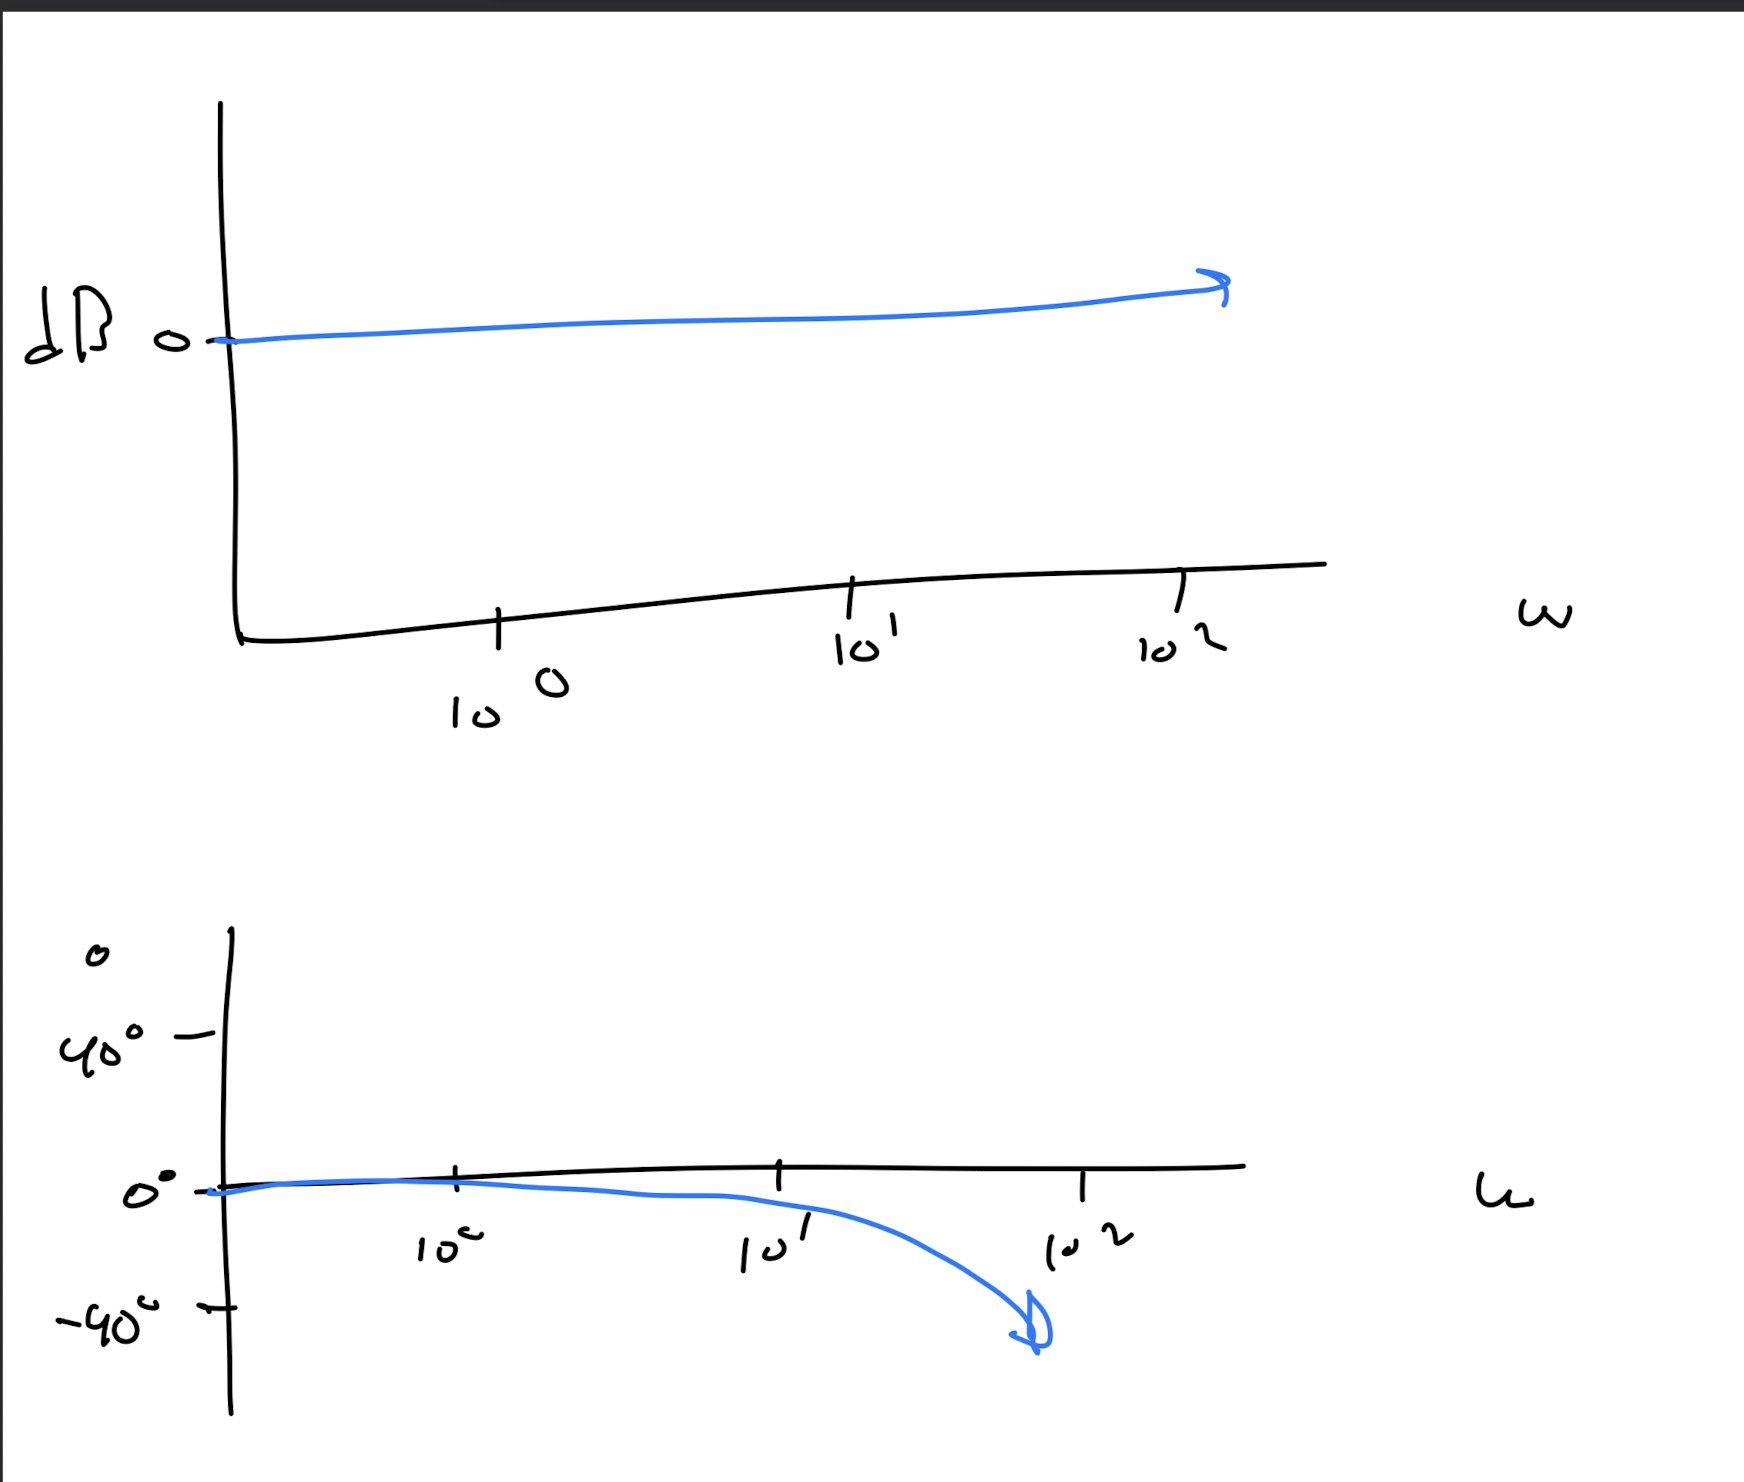
\includegraphics[width=300pt]{a2_q3.png}

\subsection{c}

$H(s) = e^{-\tau / s}$. Taking the Laplace transform of the input, $U(s) = \dfrac{0.15 \times 2 \pi}{s^2 + (2\pi)^2}$. The output is given by $Y(s) = H(s) U(s) = \dfrac{0.15 \times 2 \pi e^{-\tau / s}}{s^2 + (2\pi)^2}$. Taking the inverse Laplace transform, we get apply the rules for sin and time shifting to get $y(t) = 0.15 \times \sin (2\pi (t - \tau))$.

\subsection{d}

Yes it holds because the output is a sinusoid with a modified amplitude that has been phase shifted, but at the same frequency.

\end{document}
